\newpage
\chapter{Experimental Results}
\label{experiment_results}
\lhead{\emph{Experimental Results}}
We first present a full replication and extension of the work by \citet{radDeliberationSinglePeakednessCoherent2021}. Then we present the simulations based on our model of meta-deliberation, as well as the results of the sensitivity analysis on both models. All code for the replication, main experiment and visualization can be found in this \href{https://github.com/amirsahrani/master_thesis}{Repository}.


\section{Replication}
We are able to fully replicate the results found by \citet{radDeliberationSinglePeakednessCoherent2021},  in \Cref{fig:rep_cyclic} we see that while the bias is less than 0.73, all metric results in a-cyclic preferences. We also replicate the behavior of the KS metric, where biases in the range of 0.73-0.85, show even some initial a-cyclic profiles can become cyclic. \Cref{fig:rep_count} Further explains this by showing that within this range we always observe 3 unique profile for the KS metric, while DP and CS have already settled on 6 profiles, thereby representing all possible preferences. \Cref{fig:rep_condorcet} shows KS introduces ambiguity in the case that there was a Condorcet winner, resulting in losing the original nice profile. Finally, the proximity to single-peakedness shows a slightly more positive note for the KS metric, showing that while the DP and CS bottom out to the minimum proximity to single-peakedness, KS stays relatively close. Though this should be taken with a grain of salt, as it is likely a consequence of the unique preferences being smaller.

\begin{figure}[htbp]
	\centering
	\begin{minipage}{0.45\textwidth}
		\centering
		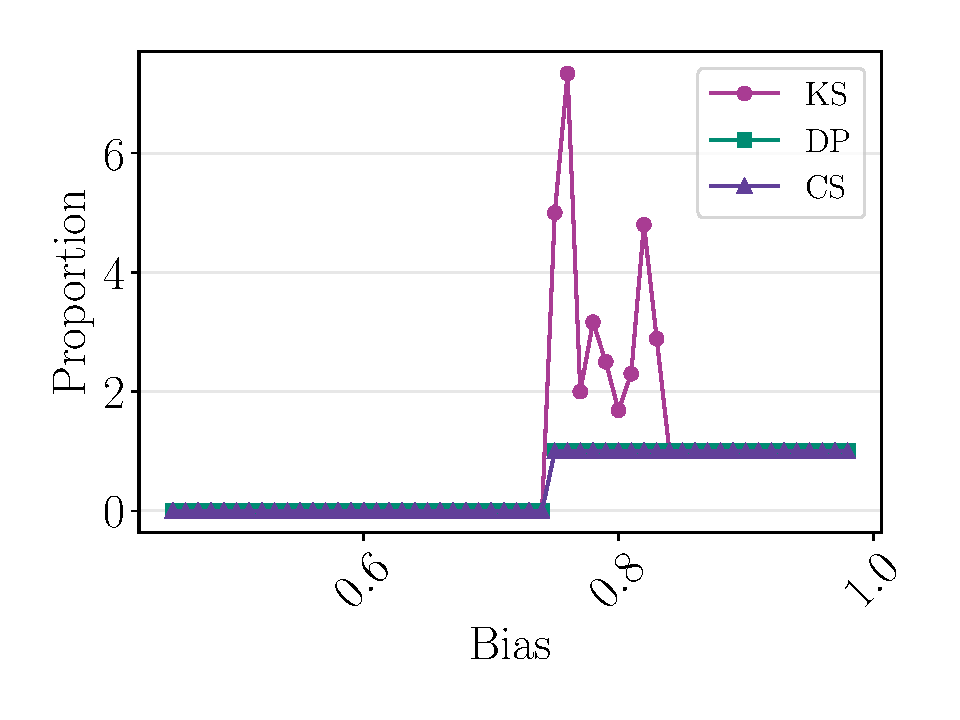
\includegraphics[width=\textwidth]{Figures/cyclic_proportion_Proportion.pdf}
		\caption{The proportion of cyclic profiles remaining, 0 indicating that no cyclic profiles were present after deliberation.}
		\label{fig:rep_cyclic}
	\end{minipage}\hfill
	\begin{minipage}{0.45\textwidth}
		\centering
		\vspace{-9pt}
		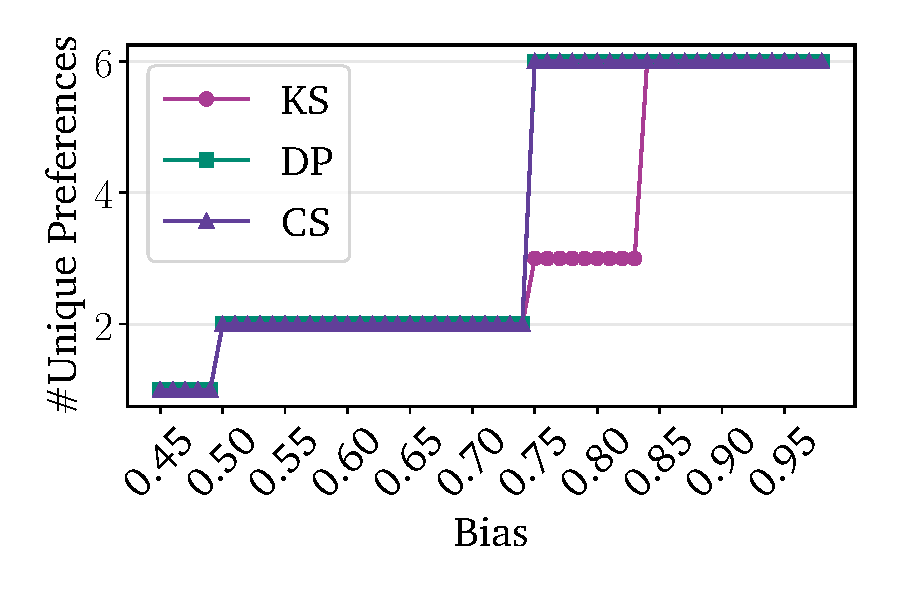
\includegraphics[width=\textwidth]{Figures/unique_Unique Preferences.pdf}
		\caption{Number of unique preferences at the final step of deliberation.}
		\label{fig:rep_count}
	\end{minipage}

	\vspace{1em}

	\begin{minipage}{0.45\textwidth}
		\centering
		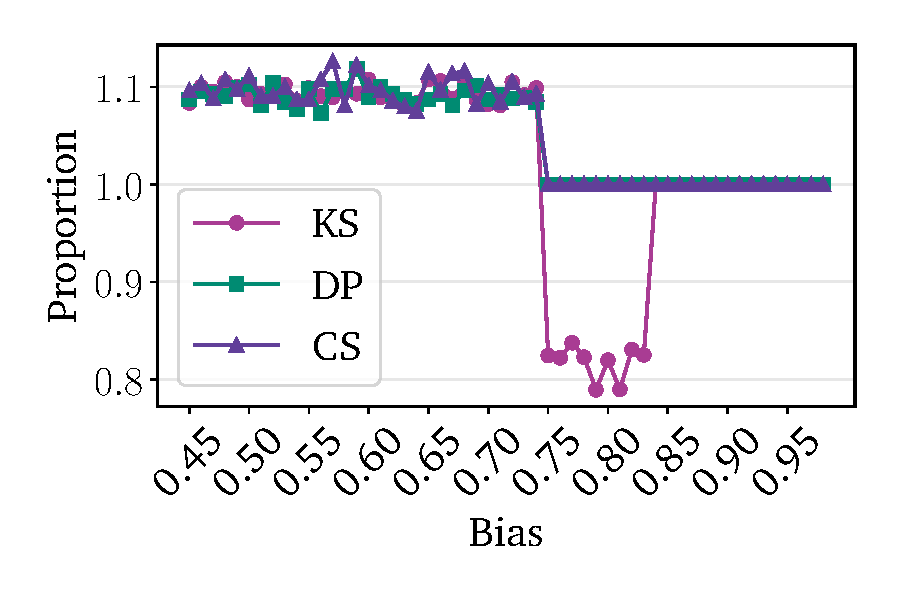
\includegraphics[width=\textwidth]{Figures/condorcet_proportion_Proportion.pdf}
		\caption{The proportion of Condorcet winners left after deliberation, value above one indicate Condorcet winners emerging during deliberation}
		\label{fig:rep_condorcet}
	\end{minipage}\hfill
	\begin{minipage}{0.45\textwidth}
		\centering
		\vspace{-9pt}
		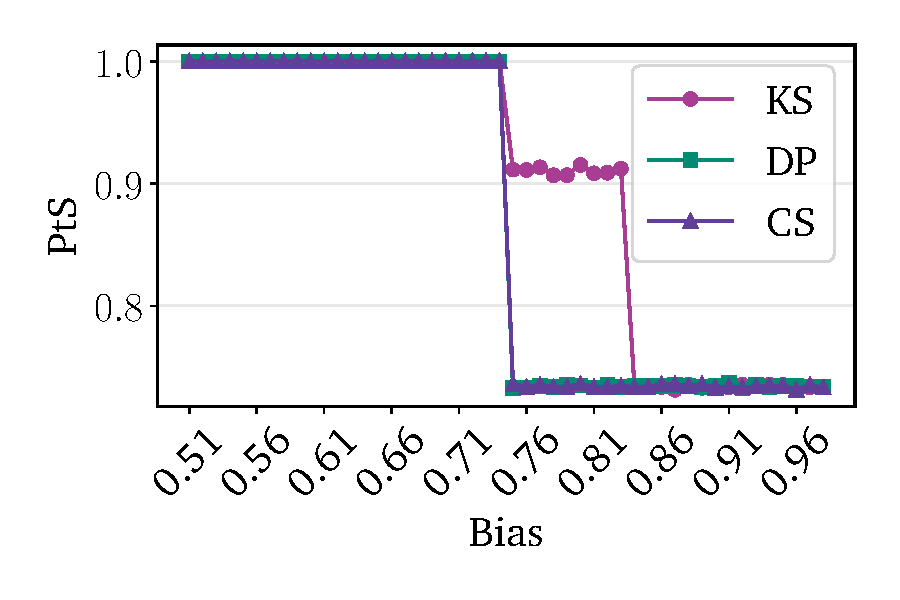
\includegraphics[width=\textwidth]{Figures/sp_proximity_PtS.pdf}
		\caption{Proximity to single-peakedness after deliberation. Proximity to single-peakedness as defined in \Cref{section:related_work}.}
		\label{fig:rep_single_peaked}
	\end{minipage}
\end{figure}
